\documentclass[11pt, oneside]{article}
\usepackage{geometry}  
\geometry{letterpaper}
\usepackage{graphicx}

\usepackage{amssymb}
\usepackage[breaklinks]{hyperref} \hypersetup{colorlinks=true,citecolor=blue,linkcolor=blue,urlcolor=blue}

\def\ICSD{{\small ICSD}}

\title{CMM HW2}
\author{Xuanhao Lin}
\date{October 1, 2023}

\begin{document}

\maketitle

\begin{figure}
    \centering
    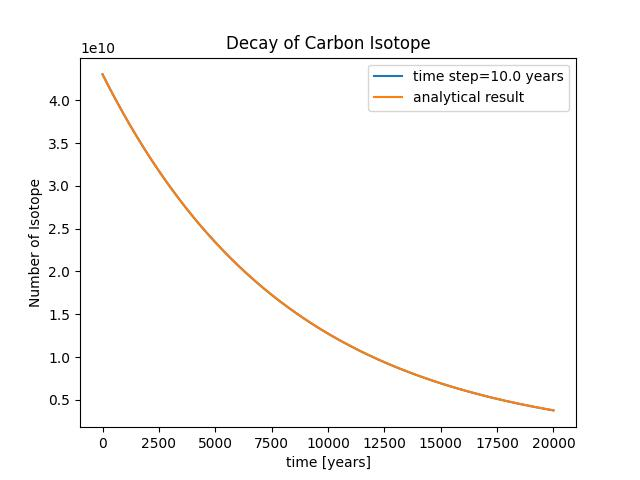
\includegraphics[width=0.5\linewidth]{Decay_of_Carbon_Isotope_with_Time_Step_Width=10.0.jpeg}
    \caption{Decay of Carbon Isotope with Time Step Width=10}
    \label{fig:1}
\end{figure}

\begin{figure}
    \centering
    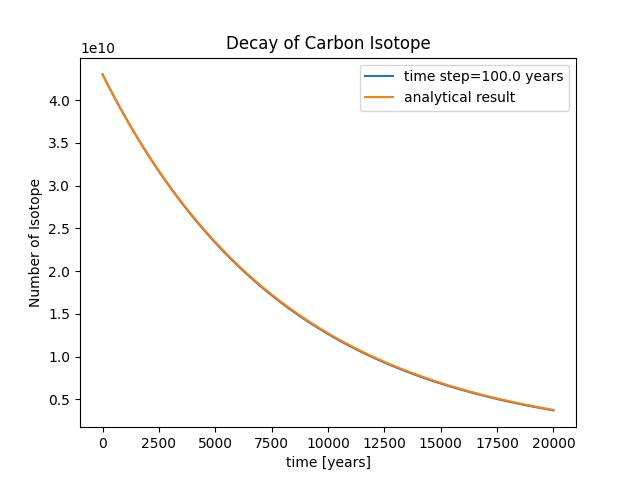
\includegraphics[width=0.5\linewidth]{Decay_of_Carbon_Isotope_with_Time_Step_Width=100.0.jpeg}
    \label{fig:2}
    \caption{Decay of Carbon Isotope with Time Step Width=100}
\end{figure}

\begin{figure}
    \centering
    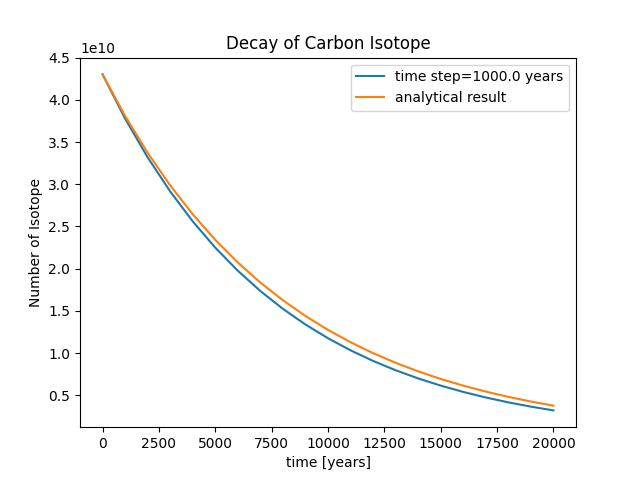
\includegraphics[width=0.5\linewidth]{Decay_of_Carbon_Isotope_with_Time_Step_Width=1000.0.jpeg}
    \label{fig:3}
    \caption{Decay of Carbon Isotope with Time Step Width=1000}
\end{figure}

\begin{figure}
    \centering
    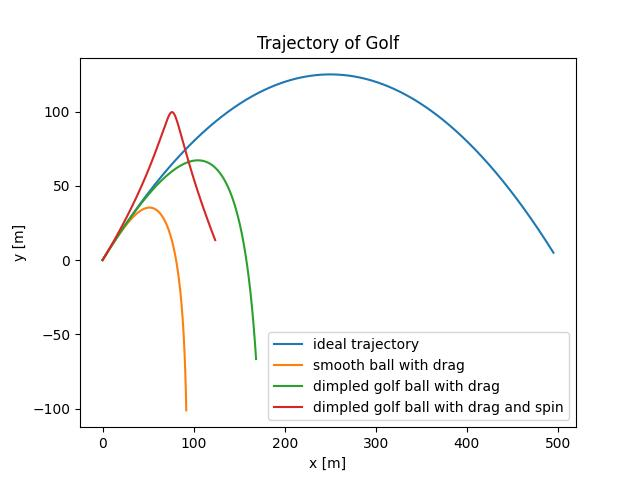
\includegraphics[width=0.5\linewidth]{Trajectory_of_Golf_with_theta=45.0.jpeg}
    \label{fig:4}
    \caption{Trajectory of Golf with $\theta=45^{\circ}$}
\end{figure}

\begin{figure}
    \centering
    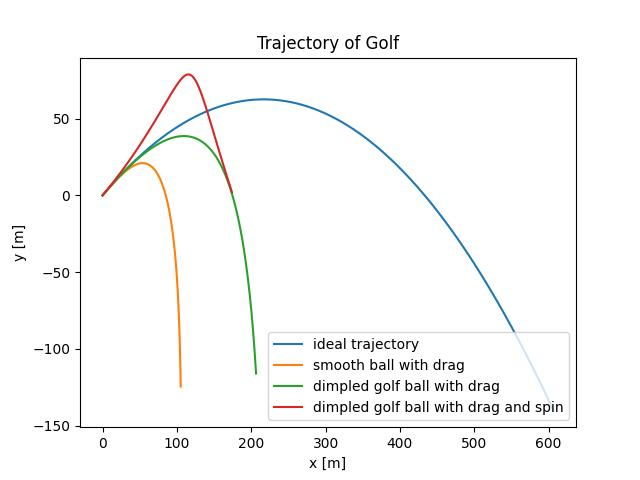
\includegraphics[width=0.5\linewidth]{Trajectory_of_Golf_with_theta=30.0.jpeg}
    \label{fig:5}
    \caption{Trajectory of Golf with $\theta=30^{\circ}$}
\end{figure}

\begin{figure}
    \centering
    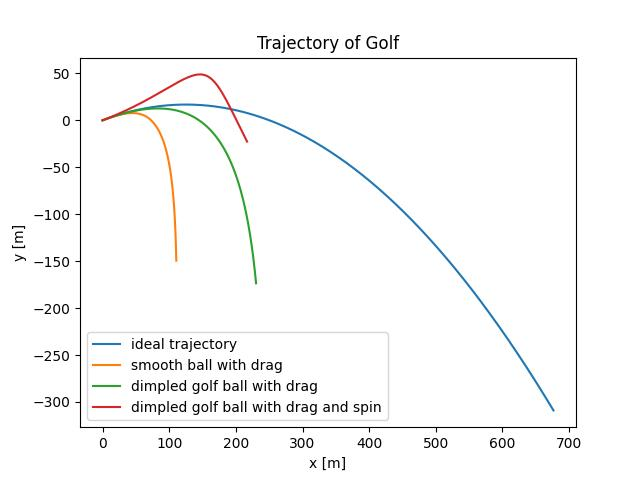
\includegraphics[width=0.5\linewidth]{Trajectory_of_Golf_with_theta=15.0.jpeg}
    \label{fig:6}
    \caption{Trajectory of Golf with $\theta=15^{\circ}$}
\end{figure}

\begin{figure}
    \centering
    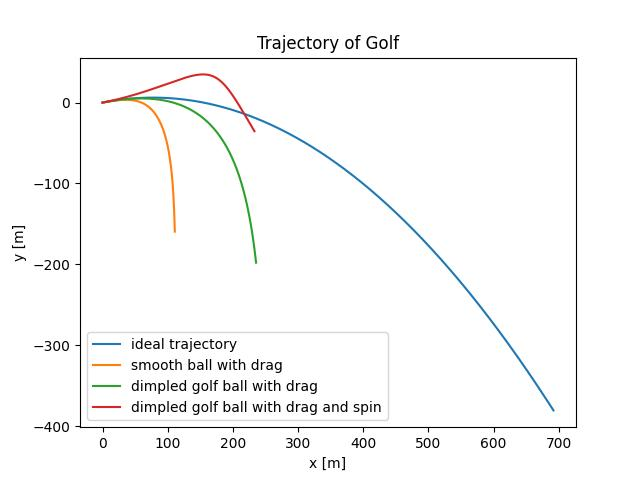
\includegraphics[width=0.5\linewidth]{Trajectory_of_Golf_with_theta=9.0.jpeg}
    \label{fig:7}
    \caption{Trajectory of Golf with $\theta=9^{\circ}$}
\end{figure}

\section{Carbon dating}
From class, we have derived the radioactive decay equation

\begin{equation}
    N(t) = N_0 e^{-\frac{t}{\tau}}
\end{equation}

Also we have half-life time of \(T_{1/2} = 5700years\). Therefore, we can calculate the decay constant $\tau$

\begin{equation}
    \tau = -\frac{5700}{\ln{\frac{1}{2}}} = 8223.36years
\end{equation}

Having calculated $\tau$, we can use numerical method to calculate the activity of the sample over a duration of 20000 years. The results are calculated by setting the time step width to values of 10 and 100 years. All results are plotted out with showing the analytical result in the same graph (\hyperref[fig:1]{Figure 1} and \hyperref[fig:2]{Figure 2}).

By increasing the time step width to 1000 years, we can find that the final values are no longer fit to the analytical results in \hyperref[fig:3]{Figure 3} since the time step width is too large. The percentage deviation of the numerical results is 14.88\%. In this case the second-order term can no longer be neglected.

\section{Golf}

According to the given values, trajectories in different cases can be plotted for different angles (\hyperref[fig:4]{Figure 4}, \hyperref[fig:5]{Figure 5}, \hyperref[fig:6]{Figure 6}, and \hyperref[fig:7]{Figure 7}). From these plots, we can clearly find that the dimpled golf can travel a longer distance in both x and y directions compared to the smooth golf when considering the drag force. However, spin can lead to different results according to the angles. We can find that the golf can travel longer distances in y direction and shorter distances in x direction with larger angles. This is because the spin can produce a magnus force which is perpendicular both motion and axis of rotation of the golf.

\section{Contribution}

This Homework shows me a clearer insight of the trajectories of the golf. Also, it helps to get a little bit more familiar with the Latex, which takes me amounts of time.

\end{document}
